\documentclass[12pt,a4paper]{article}

\usepackage{graphicx}
\usepackage{abstract}
\usepackage{wrapfig}
\usepackage{mathrsfs,amsmath} 
\usepackage{geometry}
\usepackage{fancyhdr}
\usepackage[T1]{fontenc}
\usepackage[polish]{babel}
\usepackage[utf8]{inputenc}
\usepackage{lmodern}
\usepackage{listings}
\usepackage{color}
\usepackage{xcolor}
\usepackage{hyperref}
\usepackage{subcaption}
\usepackage{multicol}
\usepackage{cleveref}
%\usepackage{siunitx}

\setlength{\headheight}{12pt} 
\setlength{\textheight}{25cm}
\setlength{\textwidth}{17cm}
\setlength{\footskip}{10mm}
\setlength{\oddsidemargin}{0mm}
\setlength{\evensidemargin}{0mm}
\setlength{\topmargin}{0mm}
\setlength{\headsep}{10mm}

\lstdefinestyle{mystyle}{
    backgroundcolor=\color{backcolour},   
    commentstyle=\color{codegreen},
    keywordstyle=\color{magenta},
    numberstyle=\tiny\color{codegray},
    stringstyle=\color{codepurple},
    basicstyle=\footnotesize,
    breakatwhitespace=false,         
    breaklines=true,                 
    captionpos=b,                    
    keepspaces=true,                 
    numbers=left,                    
    numbersep=5pt,                  
    showspaces=false,                
    showstringspaces=false,
    showtabs=false,                  
    tabsize=2
}
 
\definecolor{codegreen}{rgb}{0,0.6,0}
\definecolor{codegray}{rgb}{0.5,0.5,0.5}
\definecolor{codepurple}{rgb}{0.58,0,0.82}
\definecolor{backcolour}{rgb}{0.95,0.95,0.92}
\lstset{style=mystyle}

\selectlanguage{polish}

\newgeometry{rmargin=2.5cm,lmargin=2.5cm,bmargin=2.5cm}
\pagestyle{fancy}
\rhead{Zagadnienia}
\chead{}
\lhead{}
\lfoot{}
\cfoot{\thepage  }
\rfoot{}

\begin{document}

\thispagestyle{empty}
\begin{center}
{\Large \textbf{Egzamin Fortran}}
\end{center}
\newpage
\tableofcontents
\newpage
\section{Opracowanie zagadnień}

\subsection{Reguły zapisu instrukcji w Fortranie77}
\begin{itemize}
\item Kolumna 1 : znak C, c lub * oznacza linię komentarza i nie mają
wpływu na wykonanie programu. Komentarze można
umieszczać także po 72 kolumnie lub na prawo od znaku!
\item Kolumny 1-5 : etykieta (ciąg maksymalnie pięciu cyfr, co najmniej
jedna niezerowa; umożliwia odwołanie się do etykietowanej
linii w programie)
\item Kolumna 6 : dowolny znak (różny od zera i spacji) oznacza
kontynuację poprzedniej linii. jedna instrukcja może składać
się maksymalnie z 20. linii (wierszy)
\item Kolumny 7-72 : instrukcje FORTRANu
\end{itemize}

\subsection{Postacie stałej rzeczywistej. Podać przykłady}
\begin{lstlisting}[language=Fortran, caption=dyrektywa implicit]
REAL :: x !12.0, -.3, 1.35E-1
\end{lstlisting}
\input{sections/2}
\input{sections/3}
\input{sections/4}
\subsection{Postać stałej podwójnej precyzji. Podać przykłady}
\begin{lstlisting}[language=Fortran, caption=dyrektywa implicit]
double precision :: foo !3.54D0, 35.4D-1
\end{lstlisting}

\subsection{Na czym polega reguła pierwszej litery}
\label{sec:lit}
Jeśli zmienna nie zostanie zadeklarowana to Fortran77 przyjmie
regułę pierwszej litery w nazwie.
\begin{itemize}
\item Zmienna o nazwie zaczynające się od i, j, k, l, m, n zostaje
automatycznie przypisana do typu INTEGER
\item pozostałe do typu REAL.
\end{itemize}

\subsection{Podać przykład zastosowania dyrektywy IMPLICIT}
\begin{lstlisting}[language=Fortran, caption=dyrektywa implicit]
program test
	implicit none
	integer :: a, b, c
	...
end program
\end{lstlisting}
\subsection{Co musi wystąpić po dyrektywie IMPLICIT NONE?}
Deklaracja stałych (anuluje regułę pierwszej litery (\ref{sec:lit}))
\subsection{Sposoby deklaracji wymiaru i rozmiaru tablicy (zmiennej indeksowanej). Jaki jest maksymalny wymiar tablicy?}
Maksymalny 7-wymiarowa tablica.\\
\begin{itemize}
\item \textbf{TYP <nazwa> DIMENSION <nazwa>(n1:m1,n2:m2)}
\item \textbf{TYP <nazwa>(n1:m1,n2:m2)}
\end{itemize}


\subsection{Jaka jest różnica między funkcjami wewnętrznymi ATAN i ATAN2?}
\begin{itemize}
\item ATAN(x) - arctg w radianach
\item ATAN2(x,y) - x,y-wspł. wektora, wynik w radianach
\end{itemize}
\subsection{Wymień operatory arytmetyczne i kolejność ich wykonywania}
Zgodnie z priorytetem(jeśli równoważne to od prawej strony):
\begin{itemize}
\item potęgowanie "A**B"
\item mnożenie "A*B", dzielenie "A/B"
\item dodawanie, odejmowanie
\end{itemize}
\subsection{Wymień operatory relacji}
\begin{itemize}
\item .LT.
\item .LE.
\item .EQ.
\item .NE.
\item .GE.
\item .GT.
\end{itemize}
\subsection{Wymień operatory logiczne}
\begin{itemize}
\item .NOT.
\item .AND.
\item .OR.
\item .EQV.
\item .EQV. rownoważność
\item .NEQV.
\end{itemize}
\begin{figure}[h!]
\centering
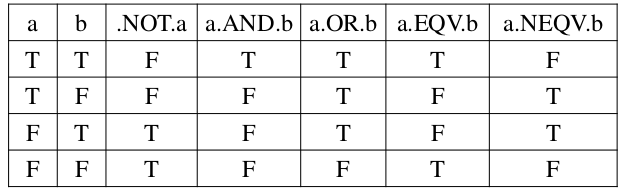
\includegraphics[scale=0.4]{oplog}
\end{figure}
\subsection{Podaj typ wyniku i jego wartość: 2/4, 2./4, 2d0/4, 5/2, 2./5}
2/4=0, 2./4=0.500000000, d20/4=0.50000000000000000, 5/2=2, 2.5=0.400000006


\subsection{Podaj postać bezwarunkowej instrukcji skoku}
\textbf{GO TO <etykieta>}
\begin{lstlisting}[language=Fortran, caption=cos]
10	n = n + 1
	go to 10
\end{lstlisting}

\subsection{Podaj postać instrukcji warunkowej prostej}
IF (wyrazenie logicze) instrukcja
\begin{lstlisting}[language=Fortran, caption=cos]
	if (foo.LE.2) bar=2
\end{lstlisting}

\subsection{Podaj postać blokowej instrukcji warunkowej}

\begin{lstlisting}[language=Fortran, caption=cos]
IF ( wyrazenie logiczne ) THEN
...
...
END IF
\end{lstlisting}

\subsection{Podaj postać instrukcji warunkowej złożonej}

\begin{lstlisting}[language=Fortran, caption=cos]
IF ( wyrazenie logiczne ) THEN
...
ELSE IF (warunek) THEN
...
ELSE
...
END IF
\end{lstlisting}

\subsection{Podaj postać arytmetycznej instrukcji warunkowej}

\begin{lstlisting}[language=Fortran, caption=cos]

\end{lstlisting}

\subsection{Podaj postać instrukcji cyklu}

\begin{lstlisting}[language=Fortran, caption=cos]
DO iterator=start, stop, step
...
...
END DO 
\end{lstlisting}

\subsection{Co to jest urządzenie standardowe? Podaj postać instrukcji czytania danych z urządzenia standardowego}
urzadzenie wejscia-wyjscia umozliwiające komunikację między programem a srodowiskiem zewnętrznym(dysk, ekran ...)

\begin{lstlisting}[language=Fortran, caption=cos]
open(10, file="cache.txt", status="old")
read(10,*) foo
close(10)
\end{lstlisting}

\subsection{Podaj postać instrukcji pisania wartości tablicy jednowymiarowej z wykorzystaniem listy cyklu (DO implikowanego)}
\begin{lstlisting}[language=Fortran, caption=cos]
program X
dimension T(3)
do j=1,3
  T(j) = float(j**2)
  write(*,*) T(j)
  do i=1,2
    
end do
end program
\end{lstlisting}


\input{sections/6}
\input{sections/7}
\input{sections/8}
\input{sections/9}
\input{sections/10}
\input{sections/11}
\input{sections/12}
\input{sections/13}
\input{sections/14}
\input{sections/15}
\input{sections/16}
\input{sections/17}
\subsection{Podaj postać arytmetycznej instrukcji warunkowej}
IF(wyrażenie arytmetyczne) etyk1, etyk2, etyk3
\\
\\
Przekierowanie obliczeń do instrukcji oznaczonej odpowiednią etykietą następuje, gdy:
\\
wyrażenie arytmetyczne<0 -> etyk1
\\
wyrażenie arytmetyczne=0 -> etyk2
\\
wyrażenie arytmetyczne>0 -> etyk3
\\
\\
przykład:
\\
\\
if(delta) 10,20,30
\\
10 print *,'brak rozwiazań'
\\
	go to 100
\\
20 print*,'jedno rozwiązanie'
\\
	go to 100
\\
30 print *,'dwa rozwiązania'
\\
	go to 100
\\
100 continue
\input{sections/19}
\input{sections/20}
\input{sections/21}
\subsection{W jaki sposób przekazywane są parametry wejściowe do segmentu function}
-podprogram może być wykonywany z danej jednostki programowej wielokrotnie z różnym zestawem danych.
\\
\\
-funkcja jest wywoływana poprzez podanie jej nazwy wraz z listą parametrów aktualnych ujętych w nawiasy okrągłe.
\\
\\
postac: 
\\
zmienna=nazwa(lista parametrów aktualnych)

\subsection{Ile watrości może być wyznaczonych w segmencie function i jak są zwracane do modułu nadrzędnego}
-w segmencie function może być wyznaczony jeden element.
\\
\\
postać:
\\
typ function nazwa (lista parametrów formalnych)
\\
deklaracje
\\
część wykonawcza
\\
nazwa=zwracana wartość
\\
return
\\
end
\\
\\
-instrukcja return powoduje zakończenie wykonywania programu i przekazania sterowania do segmentu z, którego następuje jej wywołanie.

\subsection{W jaki sposób przekazywane są parametry wejściowe do procedury subroutine}
Procedura wywoływana jest w następujący sposób:
\\
call nazwa(lista parametrów aktualnych)
\\
gdzie parametry aktualne to parametry wejściowe.

\subsection{Ile wartości może być wyznaczonych w procedurze subroutine i jak są zwracane do modułu nadrzędnego}
-procedura pozwala na zwracanie większej liczby wartości niż jedna.
\\
\\
-procedura nie ma określonego typu.
\\
\\
ogólna postać:
\\
subroutine nazwa (lista parametrów formalnych)
\\
deklaracje
\\
część wykonawcza
\\
return
\\
end
\\
\\
instrukcja return powoduje zakończenie wykonywania programu i przekazania sterowania do segmentu z, którego następuje jej wywołanie.
\subsection{W jaki sposób wartości zmiennych określone w jednym segmencie mogą być dostępne w innym module}

-takie zmienne można uwspólnić poprzez umieszczenie ich na liście obszarów wspólnych.
\\
\\
-obszar ten musi pojawić się w części deklaracyjnej segmentów, pomiędzy którymi są uwspólnione umieszczane w nim zmienne.
\subsection{Podaj postać deklaracji COMMON}
common /nazwa/ zmienna1, zmienna2
\\
\\
-zmienne mogą być proste lub tablicowe.
\\
\\
jeden obszar może być bez nazwy.
\\
\\
nazwy zmiennych mogą być inne taka sama musi być naza obszaru wspólnego i jego długość.
\subsection{W różnych segmentach może wystąpić deklaracja COMMON o tej samej nazwie. Co można powiedzieć o zmiennych wyszczególnionych w tych deklaracjach}
- Jeżeli nazwy zmiennych są inne ale nazwa obszaru wspólnego i jego długość jest taka sama, to zmienne o tej samej liczbie porządkowej są sobie równoważne.
\subsection{Jaki jest cel stosowania segmentu BLOCK DATA}
-Poprzez segment block data mogą być wprowadzane dane do programu.
\\
\\
-segment ten służy do nadawania wartości początkowych zmiennym umieszczonym w obszarach wspólnych.
\\
\\
struktura: 
\\
BLOCK DATA nazwa
\\
common /nazwa obszaru/ X,Y,I(10)
\\
data x,y,I /0.0,5.92,4*3,6*0/
\\
end
\subsection{Podać postać i cel stosowania instrukcji INCLUDE}
postać: include `nazwa pliku'
\\
\\
cel: służy do dołączenia do pliku fortranowskiego innego pliku zawierającego procedury, funkcję czy bloki danych.

\newpage
\listoffigures
\renewcommand{\lstlistingname}{Kod źródłowy}
\renewcommand{\lstlistlistingname}{\lstlistingname}
\lstlistoflistings

\end{document}
